\chapter{REVISÃO DA LITERATURA}
\thispagestyle{empty}

\section{Projetos}

\citeonline[p. 8]{meredith2011project} definem que projetos tratam da realização de tarefas específicas e finitas, de grande ou pequena escala, com um prazo de execução e um orçamento estipulado. \citeonline{turner2014handbook}, por sua vez, dispõe que projetos são tarefas com uma data final, onde caso esta data não implique na entrega do projeto, será estabelecida uma entrega do produto presente e a criação de outro projeto para entregar as tarefas restantes, referente a este produto.

Para \citeonline{kerzner2013project} um projeto pode ser caracterizado por uma série de atividades e tarefas realizadas com um objetivo específico para serem completadas sob determinadas especificações. Essas atividades e tarefas também devem possuir datas definida para inicio e fim; limites de recursos e custos; bem como um quantitativo de pessoas e equipamentos que será envolvido nestas.

Finalmente, de acordo com o \citeonline{pmiguide2014}, um projeto pode ser compreendido por um esforço temporário empreendido a fim de criar um produto, prestar serviço ou trazer um resultado exclusivo. Esse esforço é composto por um conjunto de atividades inter relacionadas e direcionadas à obtenção de um ou mais produtos únicos, com tempo e custos definidos. Nesta definição, algumas características básicas do projeto devem ser destacadas:

\begin{itemize}
  \item{\textbf{Delimitação temporal:} datas específicas para início e fim;}
  \item{\textbf{Objetivos:} metas definidas em função de um problema, oportunidade ou interesse da organização;}
  \item{\textbf{Elaboração progressiva:} etapas contínuas de desenvolvimento e incrementos;}
  \item{\textbf{Incerteza:} a representação do degrau entre o resultado esperado e as condições de realização do projeto;}
  \item{\textbf{Singularidade:} a representação da exclusividade do projeto, aquilo que o torna único;}
  \item{\textbf{Relação fornecedor-beneficiário:} relação entre quem desenvolve e quem recebe o projeto.}
\end{itemize}

Assim, pode-se compreender que todo projeto é essencialmente temporário e único, ou ainda, finito e regular, que visa o desenvolvimento de um novo produto ou serviço exclusivo.


\section{Gestão de Projetos}

De acordo com \citeonline[p. 74]{kerzner2013project} a gestão de projetos pode ser considerada uma metodologia que consiste em um processo repetitivo usado em projetos com o objetivo de alcançar sua maturidade. Afirma-se também que qualquer metodologia, inclusive a mais simples, pode representar um caso de sucesso como prática de GP, desde que seja aceita na organização em questão. Entretanto, ao utilizar uma metodologia de GP de sucesso, a probabilidade de que a organização se destaque como entregadora de bons projetos será elevada \cite{kerzner2013project}.

Para \citeonline{pmiguide2014}, a GP implica no uso de ferramentas, técnicas e da competência de utilizar recursos como: o conhecimento de conceitos, características próprias e particulares, bem como fatores críticos de sucesso para o aprimoramento e entrega de projetos de excelência. O guia PMBOK é considerado um conjunto das melhores práticas de GP, que se encontra dividida em cinco grupos de processos e dez áreas de conhecimento \cite{pmiguide2014}.

São os grupos de processos:
\singlespacing
\begin{enumerate}
  \item Iniciação;
  \item Planejamento;
  \item Execução;
  \item Monitoramento e Controle;
  \item Encerramento.
\end{enumerate}
\onehalfspacing

Quanto as áreas de conhecimento, constam os gerenciamentos de:

\singlespacing
\begin{enumerate}
  \item Integração;
  \item Escopo;
  \item Tempo;
  \item Custos;
  \item Qualidade;
  \item Recursos Humanos;
  \item Riscos;
  \item Comunicação;
  \item Aquisições;
  \item Partes Interessadas.
\end{enumerate}
\onehalfspacing


A Figura~\ref{processos_areas_pmbok} representa a divisão da relação das àreas de conhecimento pelos grupos de processos.

\begin{figure}[ht]
  \centering
  \scalebox{0.3}{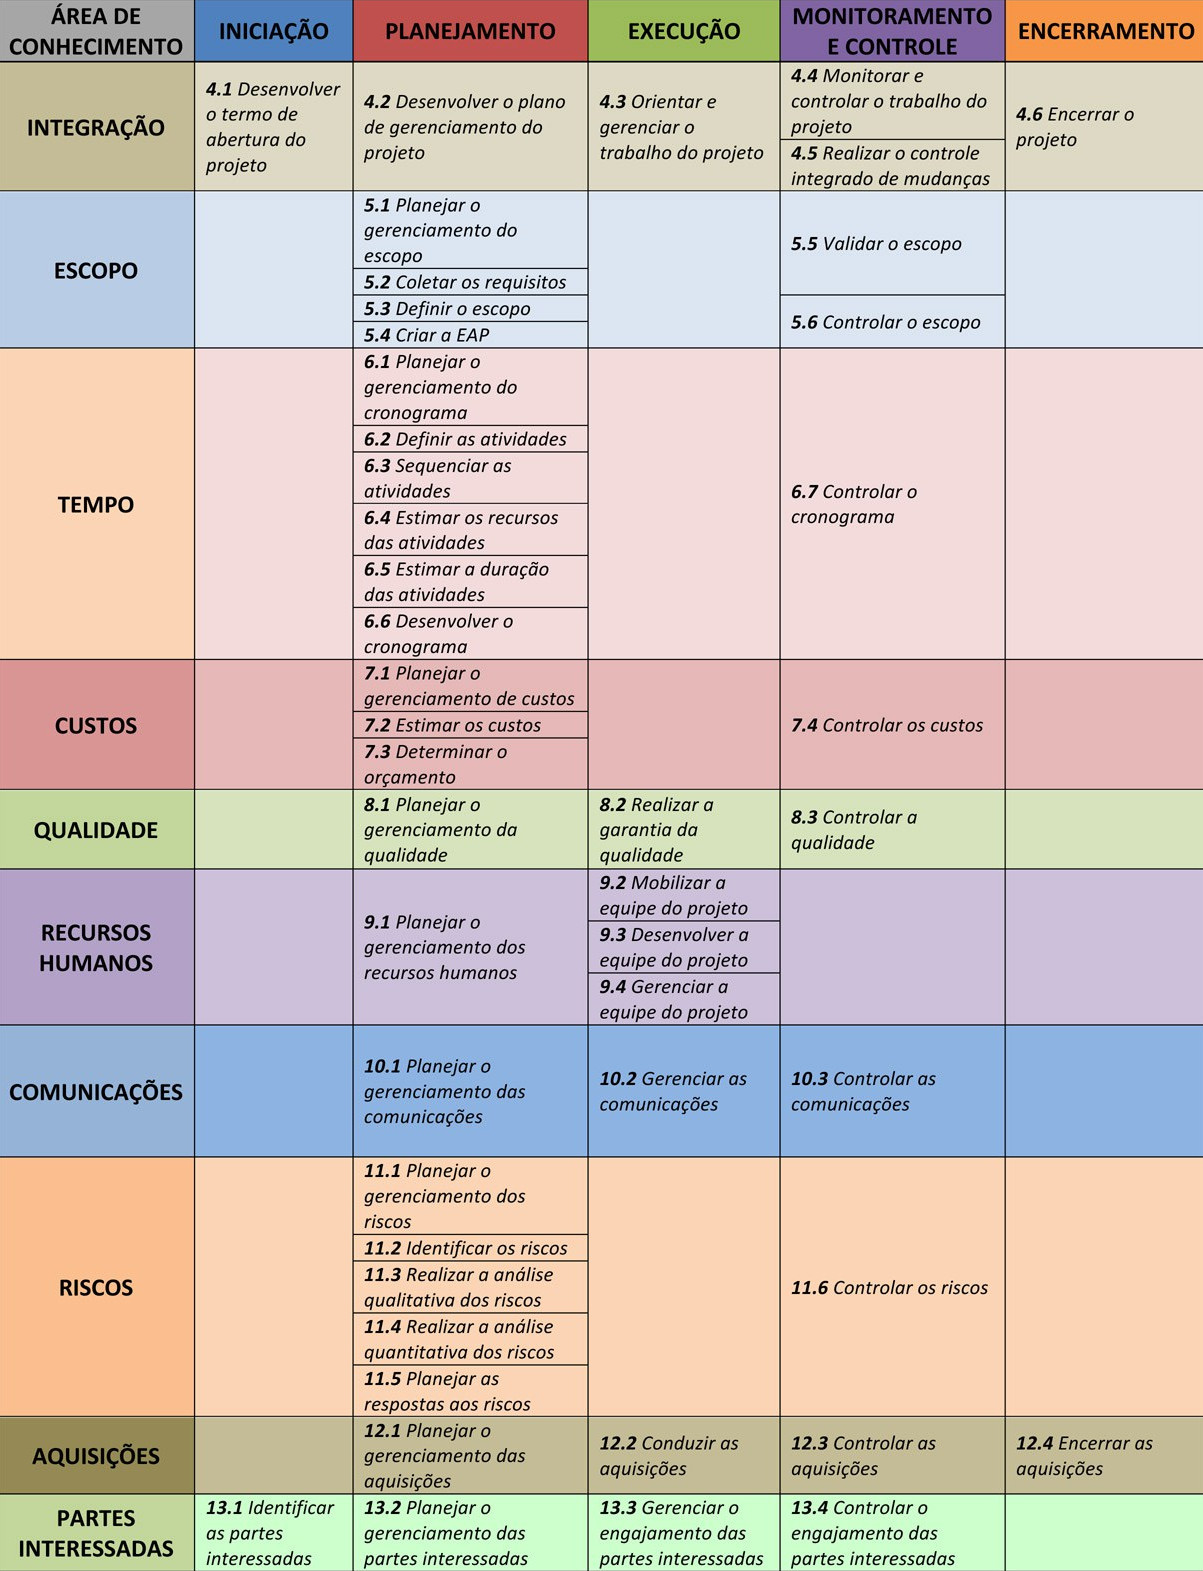
\includegraphics{figuras/processos_areas_pmbok}}
  \caption{Relação dos grupos de processos pelas àreas de conhecimento. Fonte: \cite{pmiguide2014}}
  \label{processos_areas_pmbok}
\end{figure}

Alguns autores afirmam que a garantia de que os objetivos definidos de projeto serão alcançados depende de um processo disciplinado, por parte da GP, que respeite custos, prazos e desempenho requeridos e que ocorra através do envolvimento de pessoas em atividades de planejamento e controle numa organização \cite{dinsmore2009ama, meredith2011project}.


\section{Sistemas de Gestão de Projeto}

Ao contrário do que é esperado pela natureza de negócios ou operações usuais, a natureza dos projetos e serviços é representada por processos curtos, repetitivos e funcionais, que facilitam a identificação de padrões usualmente inseridos em soluções de informação. Assim, especialista de GP veem o uso de sistemas de gestão de produtos (SGP), como uma ferramenta preciosa no que respeito a alcanço os objetivos e na excelência de projetos \cite{cserban2011project}.

Seguindo mais além, \citeonline{prado2006mmgp} afirma que diversos aspectos das metologias de GP dependem indiretamente do uso de SGP, sem que porém, seja determinada a natureza do SGP. O autor infere ainda que só é possível para organizações almejarem determinados níveis de maturidade se utilizarem essas ferramentas.

Através de um estudo quantitativo, \citeonline{liberatore2001project} analisou que nunca antes a adoção de uma ferramenta para auxiliar nas práticas de GP foi tão explorada quanto o uso de SGP. Os especialistas de GP demonstraram grande interesse pela facilidade encontrada no compreendimento da complexidade do projeto através desses sistemas, e expressaram interesse em integrar cada vez funcionalidades referente aos projetos.

Por meio de uma revisão na literatura \citeonline{hartmann2009implementing}, acrescentou que além de auxiliar no tratamento da complexidade nos projetos, o uso de SGP também se destaca para o aprimoramento da produtividade do processo de projeto, apesar de também ser notada uma dificuldade inicial para o adaptamento do uso dessas ferramentas.

Além de prover um meio para lidar com a produtividade de processo e complexidade do projeto, já foi comprovado também que o uso de SGP influi nos processos de planejamento, comunicação, monitoramento, controle de riscos, cronograma, gerenciamento de documentos e ainda avaliação de custos \cite{raymond2008project}.

Portanto, o uso de SGP implica em deter ferramentas capazes de facilitar e otimizar o esforço empregado pela GP para alcançar a excelência na realização do projeto, não apenas por parte do uso dos gestores do projeto, mas também por incluir outros atores presentes em seus processos \cite{cserban2011project}.


\section{Escritorio de Gestão de Projetos}

Advindo do inglês \textit{Project Management Office}(PMO), o escritório de gestão de projetos (EGP), ou ainda escritório de projetos (EP), pode ser considerado um conjunto de profissionais de GP que servem a um modelo organizacional com o propósito de aumentar a eficiência e lidar com as necessidades da GP, assumindo um papel de alta confiança ao implementar diversas estratégias em projetos \cite{kendall2003advanced}.

Através de um estudo, \citeonline{pemsel2013project} identificou três principais atividades que são esperadas do EGP:

\begin{itemize}
  \item Promover e facilitar o desenvolvimento estratégico da GP, bem como o uso estratégico de objetos que sejam empreendidos na GP;
  \item Planejar, controlar e dar suporte a GP, sempre assegurando que o conhecimento seja compartilhado no processo para melhorar sua eficiência;
  \item Adoção estratégias de treinamento, negociação e formação para prover o desenvolvimento de competências.
\end{itemize}

Para \citeonline{dinsmore2005pmo} a principal expectativa empregada por um EGP esta relacionada ao suporte e orientação; ao processo de desenvolvimento e gerenciamento de projetos mais eficiente e eficaz o possível; e ao uso de metodologias e recursos de planejamento e análise de projetos padronizadas.

De acordo com \citeonline{crawford2010strategic}, por mais simples que um EGP possa ser, suas atividades compõem estruturas complexas responsáveis por atividades de planejamento, controle e monitoramento, cuja implantação representa um processo de mudança de cultura organizacional, por estar diretamente relacionada à negociação com pessoas. O autor retrata ainda três níveis de atuação do EGP que podem ser visualizados na Figura~\ref{pmo_crawford}.


\begin{figure}[ht]
  \centering
  \scalebox{0.6}{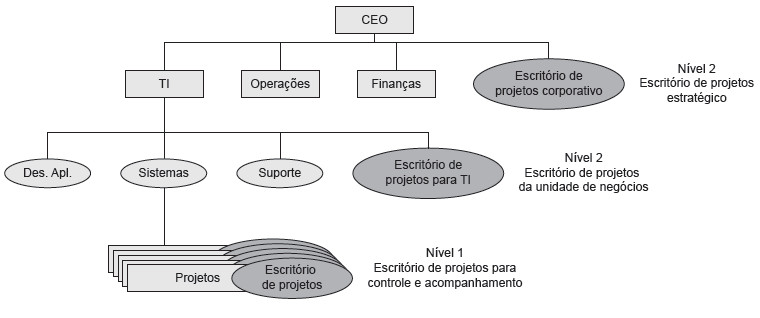
\includegraphics{figuras/pmo-crawford}}
  \caption{Níveis de atuação do escritório de projetos. Fonte: \cite{crawford2010strategic}.}
  \label{pmo_crawford}
\end{figure}

As competências desses níveis podem ser representas como \cite{crawford2010strategic}:

\begin{itemize}
  \item \textbf{Nível 1 - Escritório de Controle de Projetos:} visa o desenvolvimento do planejamento de projetos individualmente, realizando também a emissão de relatórios de progresso. Embora tenha foco em apenas um projeto, geralmente este projetos apresenta grande porte e complexidade;
  \item \textbf{Nível 2 - Escritório de Projetos da Unidade de Negócios:} oferece suporte a todos os projetos de uma área específica, porém de porte e complexidade variados;
  \item \textbf{Nível 3 - Escritório Estratégico de Projetos:} possui as seguintes competências:
  \begin{itemize}
    \item Selecionar, priorizar e garantir a integração de cada projeto para que esteja alinhado à estratégia da organização, inclusive no que respeito aos seus recursos;
    \item Desenvolver, atualizar e divulgar a metodologia de GP bem como seus conhecimentos;
    \item Converte-se em centro da gestão de conhecimento da organização através do armazenamento de informações sobre lições aprendidas;
    \item Validar estimativas de recursos realizadas pelo projetos, baseando-se em experiências anteriores.
  \end{itemize}
\end{itemize}

Assim, as responsabilidades de um EGP podem variar de acordo com a centralização empregada na organização, uma vez que está relacionada a padronização dos processos de GP. Entretanto as ferramentas e técnicas a serem empregadas ficam sob critério do gestor responsável pelo EGP \cite{pmiguide2014}.

Alguns autores, ainda, apontam o EGP como uma ferramenta de apoio para que organizações obtenham bom desempenho em GP, bom como para alcançarem seus objetivos estratégicos. Esses mesmos autores destacam que fatores comuns ligados as taxas de sucesso do EGP, em caso positivo, devem ser enfatizados, enquanto em caso negativos, devem ser evitados, configurando assim boas práticas para o sucesso do EGP \cite{andersen2007benchmarking}.


\section{Gestão de Programas}

Programas podem ser entendidos por estruturas que consistem em uma equipe principal e um conjunto de equipes de projeto que averiguam capacidade de decisão e autoridade de um membro definitivo, isto é, um gerente de programa que assegura a direção e as decisões desta estrutura. Estas estruturas visam alcançar um determinado objetivo dentro de uma estratégia.\cite{brown2008handbook}.

\citeonline{rijke20141197} avalia que apesar da dificuldade geral em distinguir um programa de um projeto, a gestão de programas deve ser considerada mais extensa que gestão de projetos, pois ela abrange áreas em que projetos singulares não se encontram. Vale ressaltar também que o gestor de programa tem hábitos mais estratégicos que podem interferir na GP \cite{lycett2004289}.

Assim, a gestão de programas tem sido cada vez mais adotada por organizações com o objetivo de implementar estratégias que integrem melhor seus projetos e ferramentas, sem permitir que o desempenho possa desorientar a natureza estratégica das decisões.


\section{Gestão de Portfólio}

A gestão de portfólio, conhecida também por Gestão de Portfólio de Projetos (GPP), surgiu a partir da necessidade de gerenciar investimentos em projetos nas organizações. Seu processo dinâmico e integrado visa avaliar o alinhamento estratégico e a viabilidade da execução simultânea de diversos projetos ao mesmo tempo. Esses projetos passam por uma introspecção que os seleciona e organiza de acordo com sua priorização em um portfólio \cite{meredith2011project, kerzner2013project}.

De acordo com \citeonline[p. 27]{burke2013project}, um portfólio pode abrigar conjuntos de projetos, programas e até mesmo outros portfólios que não precisam estar diretamente relacionados, mas que se reúnem por uma questão de otimização e controle. A Figura~\ref{port_prog_proj} ilustra a relação entre portfólio, programas e projetos.

\begin{figure}[ht]
  \centering
  \scalebox{0.4}{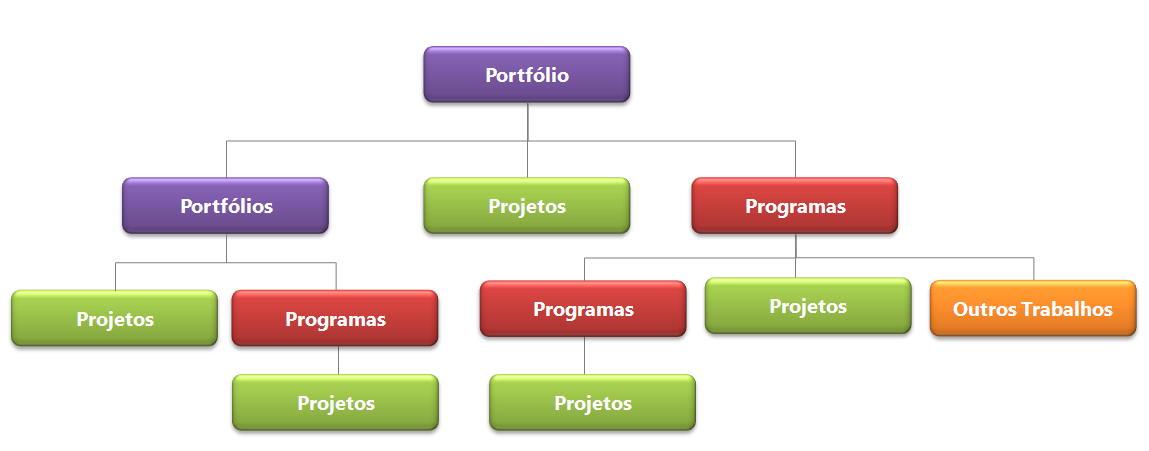
\includegraphics{figuras/port-prog-proj}}
  \caption{Relação Portfólio, Programas e Projetos. Fonte: \cite{pmi2006}}
  \label{port_prog_proj}
\end{figure}

\citeonline[p 11]{pmiguide2014} estabelece que o critério de agrupamento de um portfólio deve visar a facilitação na gestão para que seja possível atingir os objetivos estratégicos de uma organização. É definido ainda que toda gestão de portfólio fique sob responsabilidade de um EGP. A figura \ref{estrategia_portfolio} representa os processos incorporados pela Gestão de Portfólio.

\begin{figure}[ht]
  \centering
  \scalebox{0.4}{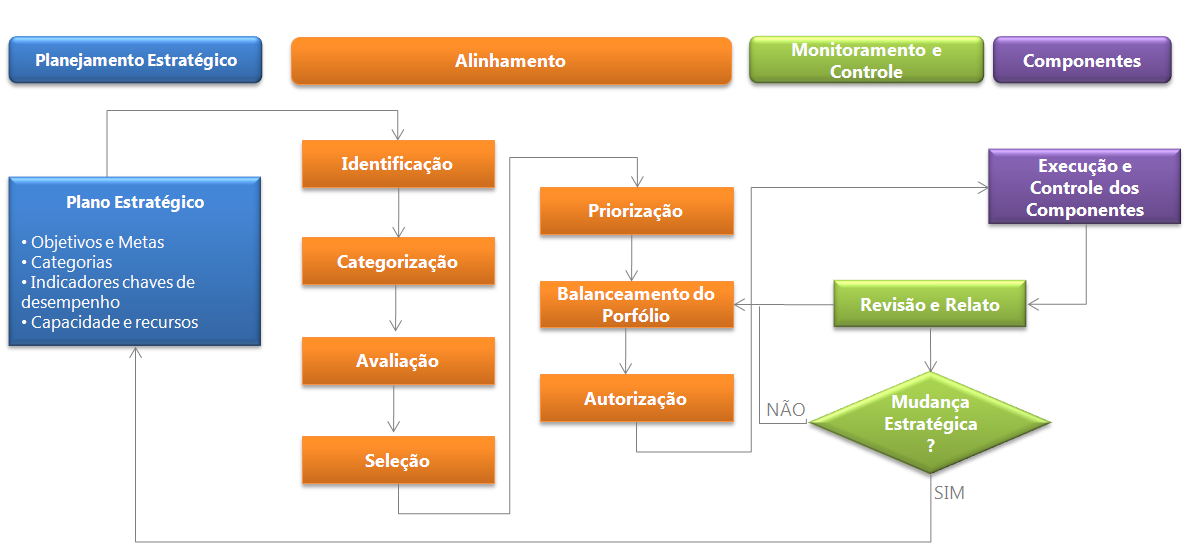
\includegraphics{figuras/estrategia-portfolio}}
  \caption{Processos de Gestão de Portfólio. Fonte: \cite{pmi2006}}
  \label{estrategia_portfolio}
\end{figure}

Desta forma, a GPP pode ser dita como uma manifestação de estratégia de negócios que determina os investimentos da organização via processos simultâneos, sistemáticos e dinâmicos de decisão, tornando o sucesso do EGP dependente do desempenho agregado de iniciativas dos componentes do portfólio e buscando a maximização do uso e do alinhamento desses componentes \cite{pmiguide2014}.

% \section{Gestão de Estratégica}
% \section{Maturidade em Gestão de Projetos}
% \section{Fatores Críticos de Sucesso}
